\chapter{Trials and failures}

\section{Machine Learning}

I've tried to create a database with the samples of current. Each sample was a vector with 50k values corresponding a 0.5s of data collected in a 100KHz oscilloscope. And in a second column its 


\subsection{Neural Network with raw data}

\subsection{Spectogram analysis}

\begin{multicols}{2}

\begin{figure}[H]
    \center
    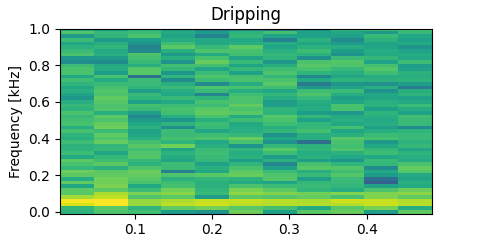
\includegraphics[width=7cm]{Figuras/spectogram/308_Dripping.png}
    \label{fig:spectrogram1}
    \caption{Dripping}
  \end{figure}

  \begin{figure}[H]
    \center
    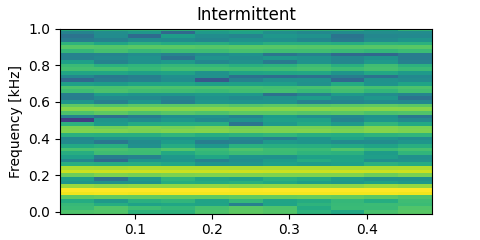
\includegraphics[width=7cm]{Figuras/spectogram/486_Intermittent.png}
    \label{fig:spectrogram5}
    \caption{Dripping}
  \end{figure}

  \begin{figure}[H]
    \center
    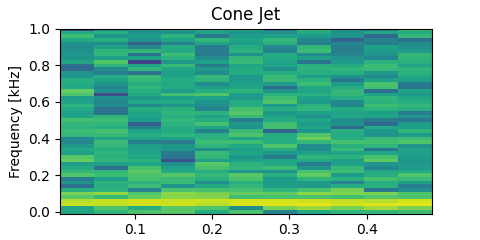
\includegraphics[width=7cm]{Figuras/spectogram/94_Cone Jet.png}
    \label{fig:spectrogram2}
    \caption{Dripping}
  \end{figure}

  \begin{figure}[H]
    \center
    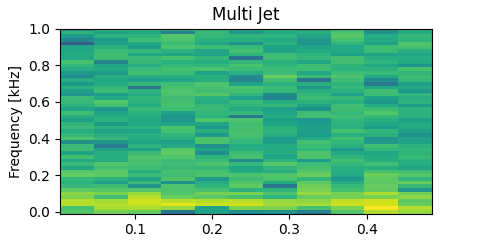
\includegraphics[width=7cm]{Figuras/spectogram/166_Multi Jet.png}
    \label{fig:spectrogram3}
    \caption{Dripping}
  \end{figure}

  \begin{figure}[H]
    \center
    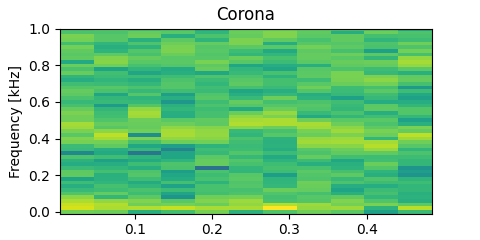
\includegraphics[width=7cm]{Figuras/spectogram/276_Corona.png}
    \label{fig:spectrogram4}
    \caption{Dripping}
  \end{figure}

\end{multicols}